\chapter{Evidence That Can Fail}
\label{ch:evidence}

A command prints the word we hoped to see. The terminal returns success. We
save the output and call it evidence. Six months later, someone changes one
byte of the claimed formula and the same command still succeeds.

The first run told us less than we thought. Perhaps the checker ignored its
input. Perhaps the command checked a proof against a different formula.
Perhaps the formula did not encode the program claim. Perhaps a shell pipeline
discarded the checker's failure code. The desired word on a screen was a fact
about one execution. It was not yet a reason to believe the theorem.

Evidence becomes useful when the route can lose. A witness checker must reject
a wrong witness. A proof checker must reject a damaged proof. A manifest
checker must notice a changed semantic package. The failure need not be
dramatic. A nonzero exit code at the right boundary is enough. What matters is
that the claimed result controls the outcome.

This chapter builds that route from first principles. We will separate tests,
complete computations, solver verdicts, certificates, and kernel
reconstruction. We will bind each result to its statement and semantics. Then
we will examine an awkward case found in an earlier generation of this very
book: a proof file almost a megabyte long that carried no load-bearing
information.

\begin{keyidea}[title={Evidence must discriminate}]
Evidence supports a claim only when a relevant change to the claim, input, or
supporting object can make its check fail. A saved success message has no such
power by itself.
\end{keyidea}

\section{Why solvers began writing proofs}

Boolean satisfiability solvers answer whether a propositional formula has an
assignment that makes it true. A satisfying answer can be accompanied by the
assignment. Another program can substitute the values and check every clause.
An unsatisfiable answer is harder: there is no assignment to hand back. The
claim ranges over all assignments, and a bare verdict asks the reader to trust
the solver's search, implementation, memory, and output path.

Proof logging changed that bargain. Instead of returning only an
unsatisfiable verdict, a solver can emit a sequence of additions and deletions
that leads to contradiction. The DRAT format became practical because it
could express the reasoning used by modern SAT solving and preprocessing,
while a separate checker could validate the log. The accompanying
\code{drat-trim} system also used backward checking and proof trimming to
reduce the portion that must be retained.\autocite{wetzler2014drat}

The next question was how much checker code the result should trust. The
linear resolution asymmetric tautology (LRAT) format adds
explicit hints to clausal steps so a simpler checker can validate them. Its
authors demonstrated certified checkers in Coq and ACL2, moving the final
decision into existing theorem-prover environments.\autocite{cruzfilipe2017lrat}
For satisfiability modulo theories, proof formats must also describe reasoning
about equality, arithmetic, arrays, bit vectors, and other theories. Alethe
grew from the proof language used by veriT toward a common interchange format
for such SMT reasoning.\autocite{schurr2021alethe}

The historical movement is not from untrustworthy software to perfect
software. It is from one opaque decision to a chain of smaller, inspectable
decisions. A proof-producing solver may be enormous and aggressively
optimized. If a much smaller checker rejects invalid proof steps, the solver
can leave the trusted base. Formula generation and semantic translation do
not disappear, however. A flawless proof of the wrong formula remains a
flawless proof of the wrong formula.

\section{Six forms of support}

The book uses six \keyterm{trust classes}: definition, trace, computation,
verdict, certificate, and kernel reconstruction. Object
\obj{EVID.def.trust-class} records these names. They describe how a result is
supported and where trust remains. They are not medals and do not form one
simple ranking for every question.
\label{def:trust-class}

\begin{figure}[htbp]
\centering
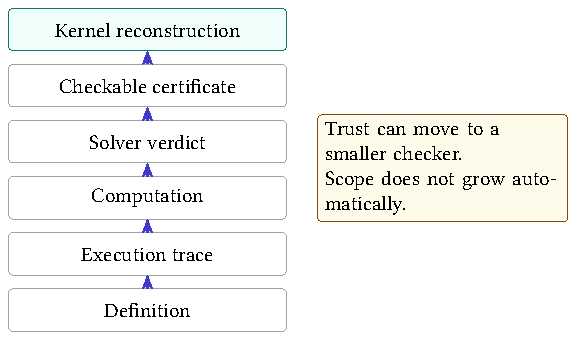
\includegraphics[width=0.94\textwidth]{figures/evidence-trust-ladder}
\caption{Six trust classes used by the book. Moving upward can reduce or
relocate trust, but no rung repairs a bad statement, semantic model, or scope.}
\figalt{A six-rung ladder runs from definition through trace, computation, verdict, certificate, and kernel reconstruction.}
\label{fig:evidence-trust-ladder}
\end{figure}

\subsection{Definition}

A definition fixes meaning. It may introduce a word, machine state, decoder,
observation, cost, or relation. Definitions need internal consistency and
clear dependencies, but they do not become empirical facts by being executed.
The A0 word set and state tuple are examples. A checker can confirm that their
records satisfy a schema; it cannot discover whether the author chose the
most useful teaching machine.

Definitions still carry a trust boundary. If a later formula implements a
different addition rule, the formula does not prove a statement about the
defined A0 instruction. Versioning and semantic digests help expose that
mismatch. They cannot decide whether the prose and formal definition express
the same intended idea. The reader remains part of the route.

\subsection{Trace}

A trace replays a particular execution. Given initial state, program bytes,
and steps, a checker can decode each instruction and confirm the next state.
This can strongly support an example or a counterexample. It does not cover
inputs absent from the trace.

Trace evidence is often the right support for an existence claim. One failing
input refutes universal equivalence. One valid two-instruction sequence
establishes an upper bound. In both cases, a small concrete object carries the
claim. The checker should still compare the complete observed state, reject an
illegal decode, and fail if any step changes.

\subsection{Computation}

A complete finite computation covers a declared domain by enumeration or a
checked recurrence. At width four, evaluating a function on all sixteen words
is complete for that width. A breadth-first search that visits every state in
a finite graph can establish reachability or its absence, provided the
transition generator and coverage test are correct.

Computation differs from testing by coverage, not by how many cases happened
to run. Ten million random tests remain samples. Sixteen cases are complete
when the domain contains exactly sixteen. A durable computation records the
domain, enumeration order or invariant, program revision, result digest, and
the condition that makes the runner fail.

\subsection{Verdict}

A solver verdict reports the result of a symbolic decision procedure. A
satisfying verdict should carry a model that can be decoded and replayed. An
unsatisfiable verdict may be reproducible by running the same or another
solver, but without a portable proof it still asks us to trust the solver and
translation route.

Agreement between two independent solvers is useful. It catches many ordinary
implementation errors. It is not the same as checking a certificate, because
the solvers may share an encoding bug, a library, or an unsupported-theory
interpretation. Report solver agreement as corroboration, not as a changed
kind of object.

\subsection{Certificate}

A \keyterm{certificate} is a finite object whose checker can validate the
claimed result without repeating the original search. A satisfying model is a
positive certificate when replay checks it. A DRAT or LRAT refutation can
certify that a propositional formula has no satisfying assignment. An Alethe
proof can record supported SMT reasoning. A rational equality or inequality
certificate can be checked with exact arithmetic.

Certificates shift trust from the producer to the checker, but only for the
statement the certificate checker receives. The checker must parse the same
formula bytes, apply sound rules, and require the claimed conclusion. A proof
format is not magic dust sprinkled on a solver log.

\subsection{Kernel reconstruction}

Kernel reconstruction translates the result into a term checked by a small
logical kernel. This can produce a theorem whose dependency footprint is
inspectable. The route is strongest when the term contains the mathematical
reasoning rather than an axiom that merely repeats the desired conclusion.

Reconstruction can also be structural. A module may import a result as an
assumption, attach provenance, and show where it is used. That is useful
attestation, but the kernel has not checked the external search. The trusted
footprint distinguishes these cases. A kernel label without that measurement
is too coarse.

\begin{warning}[title={Higher on the diagram does not mean broader}]
A kernel term for a width-four lemma may have a smaller trusted checker and a
narrower mathematical scope than a complete width-64 computation. Trust class
and claim scope answer different questions. Print both.
\end{warning}

\section{The claim must reach the checker}

An evidence route is a chain. The claim names an ISA slice, precondition,
observation, and cost. Semantic code turns instructions into state changes. A
generator translates the negated claim into a formula. A solver produces a
model or refutation. A checker validates that object. The report must bind the
result back to the original claim.

\begin{figure}[htbp]
\centering
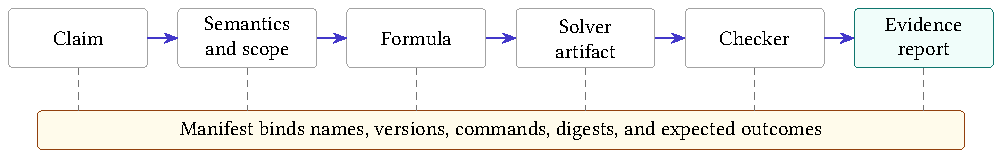
\includegraphics[width=0.97\textwidth]{figures/evidence-binding-chain}
\caption{A proof checker validates one link near the end. Digests and a
manifest bind the checked bytes to the semantics, scope, and claim that give
those bytes meaning.}
\figalt{A chain connects claim, semantics and scope, formula, solver artifact, checker, and report, with digests binding the stages.}
\label{fig:evidence-binding-chain}
\end{figure}

Every arrow admits a characteristic error.

\begin{itemize}
\item The prose may describe full architectural state while the observation
compares only one register.
\item The semantic package may reverse subtraction operands or mishandle a
partial-register write.
\item The formula generator may omit one instruction form or one cost layer.
\item The solver may return a wrong model or verdict.
\item The proof checker may accept a malformed step or never require the final
contradiction.
\item The report may point to stale bytes after a rebuild.
\end{itemize}

Testing only the final checker cannot catch all six errors. The route needs
local controls and end-to-end controls. A semantic mutation should change a
trace. A missing instruction should change the candidate-language digest. A
damaged proof should fail proof checking. A stale report should fail its hash
comparison.

\section{The evidence manifest}

An \keyterm{evidence manifest} is a small record that binds one claim to the
objects and commands used to support it. Object \obj{EVID.def.manifest}
records the book's contract. A complete manifest names:
\label{def:evidence-manifest}

\begin{enumerate}
\item the claim identifier and exact scope;
\item semantic package names, versions, and digests;
\item every input, witness, formula, proof, and result file with raw digests;
\item the producer and its configuration;
\item the checker command and expected success condition;
\item the negative control and expected failure class;
\item the trust class and any kernel footprint; and
\item limitations that remain outside the route.
\end{enumerate}

The manifest is not the evidence itself. A manifest file asserting that a proof
was checked can lie as easily as prose. Its value is binding: it tells an
independent runner which bytes to hash, which command to run, and what outcome
must change under the control.

\subsection{Raw bytes before friendly files}

Cryptographic hashes identify byte sequences. They do not identify meanings.
The book records SHA-256 digests of raw files before packaging because archive
metadata, compression headers, or regenerated line endings can change a
container without changing its mathematical content. When a compressed file
is the distributed object, record both the distributed bytes and the raw
payload when practical.

A matching hash establishes identity with the recorded bytes, not correctness.
If the original formula encoded the wrong semantics, preserving it perfectly
preserves the error. Hashes close the stale-file and substitution gaps. They
do not close the semantic gap.

\subsection{Commands need outcome contracts}

A checker command needs more than a transcript. Its process exit status must
depend on the finding. A shell command such as ``run checker, then print the
previous exit code'' is easy to misread when pipelines, timeouts, or later
commands overwrite the status. The route should execute one focused checker
and treat any unexpected result, timeout, resource exhaustion, or parse error
as failure.

Text matching deserves the same care. Searching for the substring
\code{unsat} can accept \code{not-unsat}, a diagnostic that quotes the input,
or two contradictory verdict lines. A wrapper should parse the expected
record or count exactly one anchored verdict, then test that count. The
checker, not the surrounding prose, must decide success.

\begin{example}[title={Four outcomes, only one success}]
A lower-bound check may return: the refutation is valid; the formula is
satisfiable; the proof is malformed; or the checker exceeded its resource
budget. Only the first supports the lower bound. Treating every non-satisfying
outcome as equivalent would turn a crash into mathematics.
\end{example}

\section{Negative controls}

A \keyterm{negative control} is a nearby false claim, damaged object, or
altered route that the checker must reject for a named reason. Object
\obj{EVID.prin.negative-control} records the rule that every checked route
needs one. The label \emph{negative} describes the expected result, not the
control's importance.
\label{prin:negative-control}

\begin{figure}[htbp]
\centering
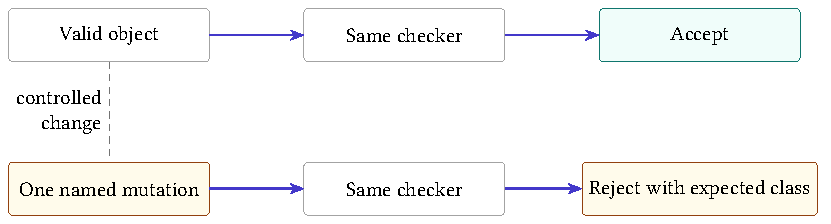
\includegraphics[width=0.94\textwidth]{figures/negative-control-anatomy}
\caption{The production object and one deliberate mutation travel through
the same checker. Acceptance on the left and the named rejection on the right
show that the route distinguishes this fault.}
\figalt{A valid object and a mutated neighbor enter one checker; one must pass and the other must fail for a named reason.}
\label{fig:negative-control-anatomy}
\end{figure}

A useful control targets a plausible failure at the same layer as the positive
claim. For a trace, change one next-state value. For a model, flip one output
bit and replay it. For a formula, add a known satisfying witness to a language
claimed empty. For a proof, delete a load-bearing step. For a manifest, change
one semantic digest. For kernel reconstruction, add one assumed law and
require the dependency footprint to contain at least one entry.

The control must share the production path. A hand-written test of a toy
parser says little about the command that checks the published artifact. Use
the same decoder, semantics, formula reader, proof checker, and wrapper wherever
the fault is meant to travel.

\subsection{Expected failure classes}

``It failed'' is not precise enough. Suppose a damaged proof also has a wrong
hash. If the manifest rejects the hash before the proof checker runs, the test
has not shown that proof checking can reject the damage. Both checks may be
valuable, but they answer different questions.

Name the expected failure class: digest mismatch, parse rejection, semantic
counterexample, illegal decode, unsupported proof rule, missing contradiction,
resource exhaustion, or nonempty kernel footprint. Then assert that the
control reached that boundary. This prevents a broken setup from impersonating
a successful control.

\begin{warning}[title={A negative control never supports the main claim}]
Correct rejection shows that the route detects one selected fault. It does not
show that the positive object is correct, that every fault is detectable, or
that the theorem's scope is right. Keep the control beside the evidence, but
do not count it as a second proof.
\end{warning}

\subsection{Positive controls matter too}

Some checkers reject everything. A negative control alone would make such a
checker look excellent. Run the production object or a known valid miniature
through the same path and require acceptance. The pair establishes one small
discrimination: this valid instance crosses the boundary and this invalid
neighbor does not.

When testing a resource limit, include a case that completes inside the
budget. When testing an unsupported proof rule, include a supported rule that
passes. When testing a semantic mutation, replay an unmutated instruction as
well. Controls work in pairs because a useful checker must distinguish, not
merely approve or object.

\section{Designing a checker as a small mathematical machine}

A checker is easiest to trust when its job can be stated as a short transition
system. Its input is a formula and a sequence of certificate steps. Its state
contains only the facts needed to judge the next step. Each accepted step must
preserve a named invariant. The final state must contain the particular fact
that closes the claim. This description is more useful than saying that the
checker is ``simple.'' A thousand lines can implement a small relation badly;
ten thousand lines can implement it with unusually clear boundaries.

For a clause proof, a \keyterm{literal} is a Boolean variable or its negation.
One useful invariant is that every clause in the active
database is either an original clause or has passed the format's admissibility
test. Deletion may remove a clause from the active database, but it must not
invent a new one. Parsing must reject malformed literals and out-of-range
identifiers. The accepting state must contain the empty clause, not merely an
end-of-file marker or a line containing a familiar word. These requirements
turn implementation review into questions with yes-or-no answers.

The same pattern applies beyond propositional logic. An arithmetic certificate
checker may accumulate polynomial identities or inequalities. A program trace
checker may update architectural state one instruction at a time. A kernel
reconstruction route may translate each external step into a term whose type
states the local obligation. In every case, ask four questions:

\begin{enumerate}
  \item What is the checker's state?
  \item Which invariant must every accepted transition preserve?
  \item Which malformed or unsupported inputs cause rejection?
  \item What exact final state licenses the reported conclusion?
\end{enumerate}

These questions also expose dangerous convenience behavior. A parser that
silently skips an unknown instruction has changed the certificate language. A
checker that replaces an unsupported theory step with a solver call has moved
the trust boundary. A wrapper that catches every exception and returns success
has erased the distinction between evidence and failure. Fail-closed behavior
means that absence, ambiguity, and unsupported cases cannot cross the
acceptance boundary.

\begin{keyidea}[title={The accepting state is part of the theorem}]
Do not define success as ``the checker finished.'' Define the exact state that
the checker must reach, and make every other termination mode distinct.
\end{keyidea}

There is a useful engineering consequence. Keep parsing, transition checking,
and reporting separate. The parser produces a typed object or a precise parse
error. The transition checker consumes only typed objects. The reporter
serializes the outcome without deciding it. This division does not establish
implementation correctness, but it makes accidental acceptance paths easier
to find and makes negative controls easier to aim.

\subsection{A hand audit before automation}

Before trusting a new checker on a large artifact, construct the smallest
example that exercises each rule. Write the expected state after every step.
Then alter one premise, one identifier, and the final step in separate copies.
The valid example should pass; each altered copy should fail for the predicted
reason. This hand audit is the certificate analogue of executing a short
instruction trace before running a whole program.

Large benchmarks test scale. They rarely isolate meaning. A million-step proof
can pass even when a rarely used rule is wrong, and its size makes diagnosis
hard. Tiny rule-directed examples supply semantic resolution; large examples
supply operational stress. A serious evidence route needs both.

\section{A proof file that carried no information}

An earlier evidence-led version of this repository contained a DRAT file of
957,982 bytes for a one-step bounded search. Axeyum's checker accepted it. The
same checker also accepted the file after its first half was deleted. The
checker was not unsound. The underlying formula already contradicted itself
under unit propagation, so the last empty-clause step was enough. Everything
before it was decoration.

To see the mechanism, begin with a tiny conjunctive normal form formula, a
conjunction of clauses in which each clause is a disjunction of literals:
\[
 F=(a)\land(\neg a).
\]
The first unit clause forces \(a\) to true. The second forces it to false.
\keyterm{Unit propagation} repeatedly applies forced single-literal clauses;
here it reaches conflict without any search or added lemma.

One common DRAT check asks whether an added clause has the reverse unit
propagation property: temporarily negate that clause, add those negated
literals as units, and see whether propagation reaches conflict. For the empty
clause there are no literals to negate. If the original formula already
conflicts under propagation, the empty clause passes immediately.

\begin{proofkit}[title={Reader argument: why the prefix is irrelevant}]
Assume a conjunctive normal form formula (F) reaches conflict by unit
propagation alone. Consider any candidate DRAT log whose final addition is the
empty clause. A backward checker tests whether that empty clause follows by
reverse unit propagation. Negating the empty clause adds no assumptions, so
the check runs unit propagation on (F) itself. By the premise, that run
conflicts. The final step is therefore accepted without using any earlier
proof step. Delete or replace the prefix and the same reason remains.
\end{proofkit}

\begin{figure}[htbp]
\centering
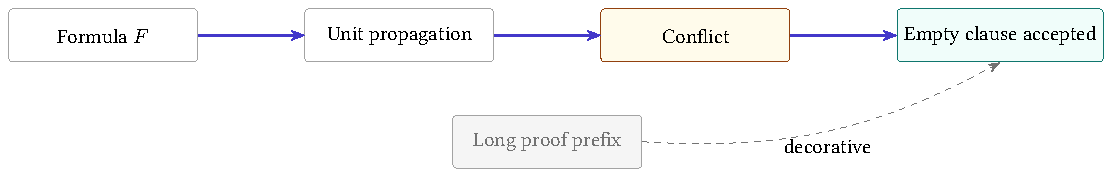
\includegraphics[width=0.93\textwidth]{figures/vacuous-proof-route}
\caption{When the original formula already conflicts under unit propagation,
the final empty clause is accepted without support from the preceding proof
steps. The formula, not the long prefix, carries the refutation.}
\figalt{A contradictory formula reaches unit conflict directly, allowing an empty clause while bypassing a long proof prefix.}
\label{fig:vacuous-proof-route}
\end{figure}

The archived formula contained 2,663 variables, not merely the two clauses
above. The structural fact was the same. A small repository script,
\code{scripts/up_refutes.py}, checks whether a standard CNF formula reaches a unit
conflict before a proof file is credited as load-bearing. The archived control
used another formula that reached a propagation fixpoint without conflict;
its actual refutation was then needed and a truncated proof was rejected.

The lesson is subtler than ``large proofs can be fake.'' The accepted proof
file was syntactically valid, and the formula really was unsatisfiable. The
mistake was attribution. The repository said the megabyte proof supported the
claim when the original clauses already contained a cheaply checkable
contradiction. The better evidence route records the unit-propagation check and
says that the proof prefix contributes nothing.

\begin{tryit}[title={Perform the vacuity check by hand}]
Run unit propagation on
\(F_1=(a)\land(\neg a\lor b)\land(\neg b)\). Then run it on
\(F_2=(a\lor b)\land(\neg a\lor b)\land(a\lor\neg b)\).
Which formula reaches conflict without a decision? For the other, give a
satisfying assignment or identify the first decision needed.
\end{tryit}

\section{Formula generation is part of the proof}

A checked refutation establishes that one concrete formula is unsatisfiable.
For a program claim, we also need to know what the variables and clauses mean.
The generator must cover every allowed candidate, implement the instruction
semantics, negate the desired equivalence correctly, and encode the chosen
cost bound.

A useful translation argument has two directions. \keyterm{Soundness of the
encoding} says that any satisfying formula assignment decodes to a real
counterexample or candidate in the declared language. \keyterm{Completeness of
the encoding} says that every real counterexample or candidate in that
language can be represented by a satisfying assignment. For a lower bound,
both directions matter. Soundness prevents spurious models; completeness
prevents the formula from silently omitting the cheaper program that defeats
the claim.

The reader proof can use a miniature. At A0 width two and program length one,
enumerate the instruction selectors and show how each selected operation
determines the next-state bits. Decode a satisfying assignment back to one
instruction and one separating input. Then explain how the production
generator repeats the same construction at the target width and bound.

Cross-checks help at this bridge. Generate tiny instances and compare the
formula's models with direct enumeration. Mutate one instruction semantic rule
and require disagreement. Count the candidate forms produced by the grammar
and compare that count with an independent expansion. These checks do not
replace a general translation theorem, but they expose the exact surface the
theorem must cover.

\section{Independent checking is a relation, not a brand}

Calling a checker independent requires a concrete account. A checker in the
same binary may still use different algorithms and parsers. A separate binary
may share the same library that contains the bug. Two tools may implement one
format from separate specifications. Independence has dimensions: codebase,
algorithm, parser, runtime, proof representation, semantic implementation,
and institutional origin.

State which dimensions differ. Axeyum's proof-producing SAT core and its DRAT
checker are separate implementations in the same repository. Its in-memory,
streaming, and file-backed checking paths can be compared, but shared clause
types and rule definitions remain part of the trust story. LRAT can move the
result to a simpler hint-following checker. Alethe output can be checked by an
external implementation only for the rules that implementation supports.
Unsupported rules must remain visible refusals, not silently trusted steps.

\begin{example}[title={Agreement can still be diagnostically valuable}]
Suppose direct enumeration, a bit-vector solver, and a SAT encoding all return
the same width-four counterexample. Their agreement does not create a formal
certificate. It does sharply localize a later disagreement at width 64: the
shared mathematical specification is less suspect than the widened encoding
or solver route.
\end{example}

\section{Kernel reconstruction and its footprint}

A kernel check is only as informative as the term and environment supplied to
the kernel. If reconstruction creates an axiom named after the desired result
and then returns that axiom, the kernel has confirmed type consistency, not
the external reasoning. The dependency footprint should list every assumption
reached by the final term.

Theory reconstruction can be stronger. A linear-arithmetic certificate may be
translated into exact rational equalities and order steps, then checked from
the kernel's arithmetic laws. A propositional LRAT proof may be replayed by a
verified checker whose soundness theorem lives in the prover. The resulting
term can have a small, measured trusted surface.

Search-based program minimality poses a further composition problem. The
kernel needs the final propositional contradiction and a link from decoded
machine programs to the generated clauses. Importing the SAT
result as an assumption does not create that link. A future A0 route may use
proof by reflection: define a small checker in the logic, run it on the
serialized language and certificate, and apply a kernel-checked soundness theorem.
Until that route exists, the manifest must distinguish checked external
evidence from kernel reconstruction with mathematical content.

\section{Resource failures are evidence outcomes}

Proof checking consumes time, memory, file descriptors, and disk space. A
certificate can be much larger than the formula and more expensive to check
than the original search. If the operating system kills the checker, no
logical verdict has been produced. Treating absence of a counterexample as a
lower bound would confuse resource exhaustion with contradiction.

The checker contract should distinguish verified, rejected, unsupported,
timed out, and resource exhausted outcomes. Only the first supports the
positive evidence row. Record budgets and peak use when they determine whether
another person can reproduce the check. For large proof streams, record
whether the checker retained the whole proof, traversed a backward core, or
used a file-backed representation.

Resource controls can fail too. A timeout wrapper must deliver termination to
the actual checker process and propagate its outcome. A disk-space preflight
must inspect the filesystem that will hold the proof. A memory estimate is not
a measurement. The workbench is part of the epistemology when its limits can
change which answers survive.

Evidence also has a maintenance cost. A certificate format may remain stable
while its checker, build system, or runtime disappears. Keep the smallest
portable artifacts that preserve the route: plain formula and certificate
files, a machine-readable manifest, checker source or a durable source
reference, and tiny controls. Containers can make reproduction convenient,
but they should package this material rather than become its only description.

When a route is rerun years later, preserve the old report beside the new one.
Do not silently replace digests or normalize away a changed outcome. The
difference may reveal a repaired checker, a changed resource limit, or an
unstable dependency. Evidence is a record of a particular discrimination at a
particular boundary; its history can itself become diagnostic evidence.

\subsection{Reproduction is a second experiment}

Reproduction should begin from the manifest, not from the author's shell
history. The person repeating the experiment obtains the named inputs and
checks their raw digests. That person then
builds or identifies the checker version, runs the declared command, and
compares the structured outcome with the contract. Only then should the person
run the negative control. This order separates an identity failure
from a checking failure and both from a control failure.

Environment capture needs judgment. Recording every installed package can
bury the dependencies that matter. Recording none can make the result
unrepeatable. Prefer a narrow executable description: operating-system and
processor assumptions when relevant, compiler or interpreter version, locked
dependencies, build command, checker digest, limits, and the exact input
digests. If nondeterminism remains, record the seed and say which outputs may
vary.

Agreement after reproduction strengthens the operational claim: another run
with the bound inputs reached the same outcome. It does not repair a wrong
formula or broaden a finite theorem. Reproduction repeats the route;
independent validation changes some part of it. The evidence report should say
which one occurred.

\section{Using Axeyum for evidence}

The live Axeyum checkout contains substantial evidence machinery. Its
propositional layer can produce and check DRAT, stream proofs, perform
backward and file-backed checking, and elaborate supported reverse-unit steps
to LRAT. Its SMT routes include Alethe production and checking for selected
theory rules. Other routes reconstruct arithmetic reasoning or report a
kernel dependency footprint. These capabilities are route-specific; no one
command turns an arbitrary ISA statement into a kernel theorem.

For the book, Rust should own evidence meaning. It should define the canonical
manifest, hash raw inputs, classify checker outcomes, run controls, and reject
unsupported trust claims. A Python interface may make the route pleasant to
teach:

\begin{codelisting}[language=python,caption={The intended shape of a future evidence inspection interface}]
# Illustrative API: the book manifest interface is not yet implemented.
record = EvidenceManifest.load("a0-add-two.json")
record.verify_digests()
record.replay_witness()
record.check_certificate()
record.run_negative_control()
print(record.trust_boundary())
\end{codelisting}

The interface should return typed outcomes rather than booleans that collapse
rejection, timeout, and unsupported proof rules. It should display the exact
claim, semantic digests, checker version, and failure class. Python may
orchestrate and explain; Rust remains the authority for parsing, checking, and
canonical serialization.

The present book repository is not at that endpoint. Object
\obj{OP.evid.manifest-checker} records the missing implementation obligation.
The active artifact tree has the schema design but no completed A0 or real-ISA
evidence package to run through it. Existing Axeyum solver machinery is a
foundation. It does not fill the semantic and manifest gaps automatically.
\label{op:manifest-checker}

\section{Where the route stops}

This chapter does not claim that a negative control proves a checker sound.
It does not claim that a certificate validates its formula generator. It does
not treat matching hashes as semantic correctness, solver agreement as a
proof, or kernel import as reconstruction.

The archived vacuous-proof case concerns one former formula and checker route.
It does not impeach DRAT. In fact, the checker behaved according to the proof
rule; the repository's interpretation was too generous. The repair is better
classification and a propagation precheck, not distrust of every short proof.

No finite collection of controls anticipates every fault. The aim is narrower
and more useful: bind the claim to exact bytes, make each checker outcome
depend on the finding, attack the likely failure boundaries, and state what
remains trusted. A machine-checked result is not the end of human judgment. It
is human judgment arranged so that more of its mistakes become visible.

\section{Exercises}

\begin{enumerate}
\item \textbf{Classify.} For each of the following, name the trust class and
nearest remaining trust boundary: five random tests, all sixteen width-four
inputs, one satisfying model, one solver verdict, one checked DRAT file, and a
kernel term with a nonempty assumption footprint.

\item \textbf{Execute.} Replay a three-step A0 trace. Change only the final
program counter and state the exact failure a complete trace checker should
report.

\item Give a satisfying assignment for
\((a\lor b)\land(\neg a\lor c)\land(\neg c)\). Explain why replaying the
assignment is easier than supporting an unsatisfiable verdict.

\item Run unit propagation by hand on
\((a)\land(\neg a\lor b)\land(\neg b\lor c)\land(\neg c)\). List the forced
literals in order and identify the conflicting clause.

\item \textbf{Prove.} Generalize the reader argument about a propagation-
refutable formula and a final empty clause. State every premise the conclusion
needs about the backward checker.

\item Construct a formula that is unsatisfiable but does not conflict under
unit propagation from the empty assignment. Explain why an actual proof or
search is needed.

\item \textbf{Break.} Remove one load-bearing clause from a tiny refutation.
Distinguish parse failure, invalid proof step, and failure to derive the empty
clause.

\item Design a negative control for a model replayer that accidentally ignores
the most significant output bit. Give a positive model and its one-bit
mutation.

\item Design a control for an A0 trace checker that updates registers correctly
but ignores instruction decoding. Ensure the control reaches the decoder
boundary rather than failing a hash check first.

\item Explain why a proof of a byte-identical formula can still fail to support
the intended theorem when the semantic package digest changes.

\item Write the minimal fields of an evidence manifest for the two-instruction
A0 witness from Chapter~\ref{ch:languages-costs}. Include scope, semantics,
observation, cost, witness, checker, and one control.

\item Two solvers return the same verdict, but both consume a formula from one
generator. Draw the shared trust boundary and name one check that adds genuine
independence.

\item A checker returns code 137 after using all available memory. Explain why
the outcome supports neither satisfiability nor unsatisfiability. Specify how
the manifest should record it.

\item \textbf{Act as the checker.} Review a command that pipes solver output
through a text search. List three ways the pipeline can return success without
establishing the intended verdict, then design a stricter wrapper contract.

\item Give separate negative controls for formula generation and proof
checking. Explain why corrupting a file hash tests neither semantic layer.

\item State soundness and completeness obligations for translating the tiny
A0 one-instruction language into a Boolean formula. Give one bug violating
each direction.

\item \textbf{Transfer.} For one selected RV64 instruction equivalence, list
the source pin, decoder, semantics, formula, model or proof, checker, and
negative controls that a complete route would bind.

\item Design the Rust and Python boundary for the future book manifest API.
Identify which layer owns canonical bytes, typed outcomes, hash checking,
display, and user convenience.
\end{enumerate}
